\section{Prácticas en laboratorios}
\label{sec:practica_lab}

El \Gls{iab} cuenta con un laboratorio especializado para la práctica de los
estudiantes de enfermería.

El laboratorio es utilizado por los alumnos desde su segundo año de formación, y
en el mismo se desarrollan todas las materias prácticas, de manera a realizar
una formación previa a las prácticas de campo explicadas más adelante.

La \fixme{cantidad}{número} de alumnos no permite \fixme{que sea
    factible}{reformular} la enseñanza individual, por ello las prácticas se
dividen en dos partes, en la primera, similar a una aula tradicional, los
alumnos se sientan y observan al profesor realizar una simulación del
procedimiento sobre un voluntario, en este punto, el profesor realiza las
observaciones que crea son necesarias para llevar a cabo la práctica
profesional, da consejos y responde a las dudas de los alumnos,
\fixme{existen}{se utilizan?} modelos del cuerpo humano utilizados para simular
algunos procedimientos, en la figura~\ref{fig:iab_veno} se observa un modelo del
brazo humano utilizado para procedimientos de venopunción.

\begin{figure}[h!t] 
\centering 
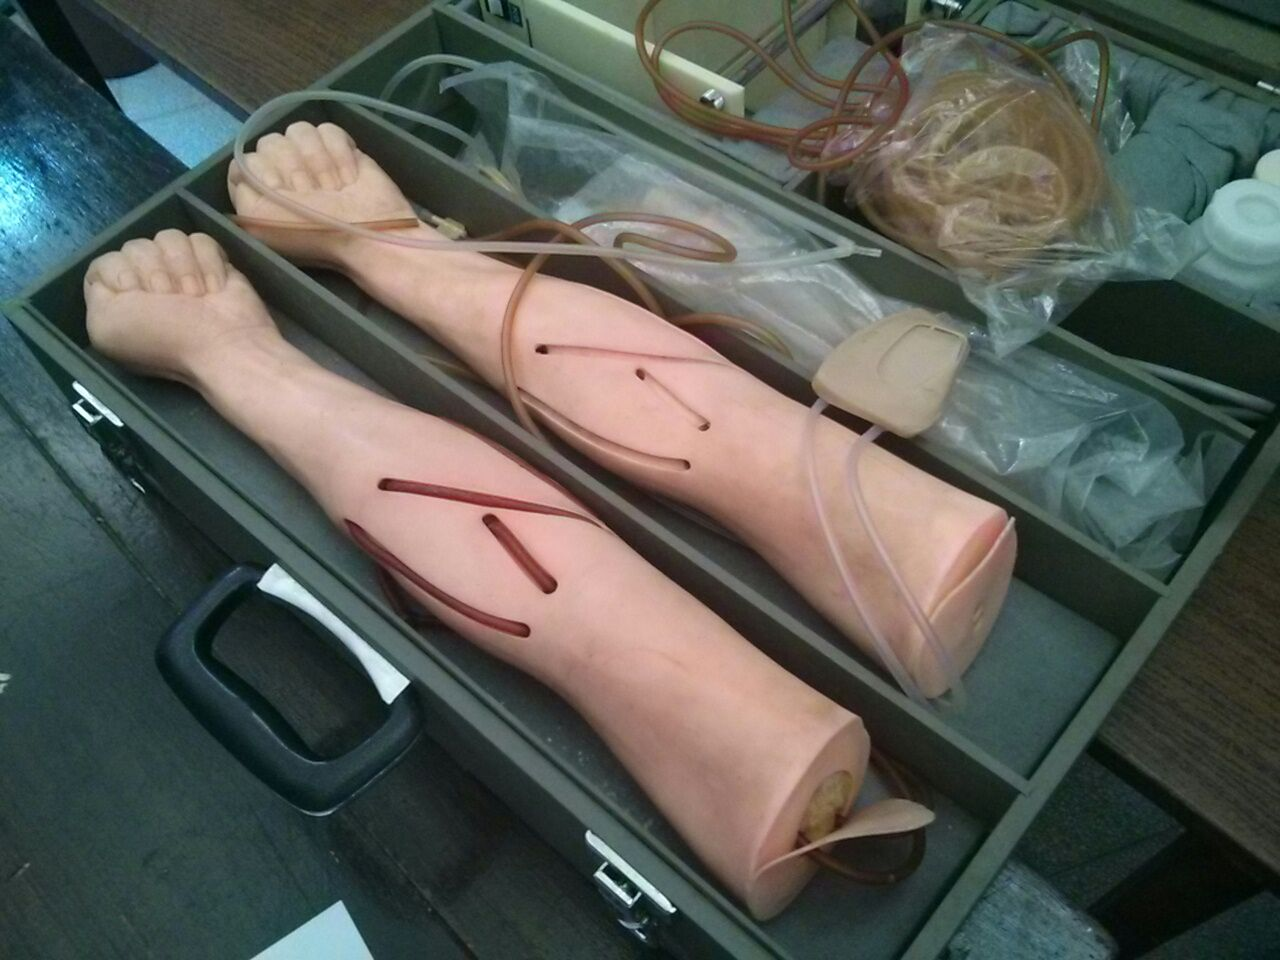
\includegraphics[scale=0.2,natwidth=100,natheight=100]{problema/iab_sala_2.jpg}
\caption{Elementos utilizados para mostrar procedimientos de venopunción}
\label{fig:iab_veno}
\end{figure}

En la segunda parte, los alumnos pasan a un laboratorio que contiene las
herramientas necesarias para la práctica (maniquís, camas de hospital, y otros
elementos, como se ven en la figura~\ref{fig:iab_lab}), donde pueden explorar y
practicar siempre bajo tutela del profesor. \fixme{Esta parte}{?} se diferencia
principalmente de la primera, en que hay más materiales para las pruebas y los
alumnos pueden realizar por sí mismos una simulación de los procedimientos.

\begin{figure}[h!t] 
\centering 
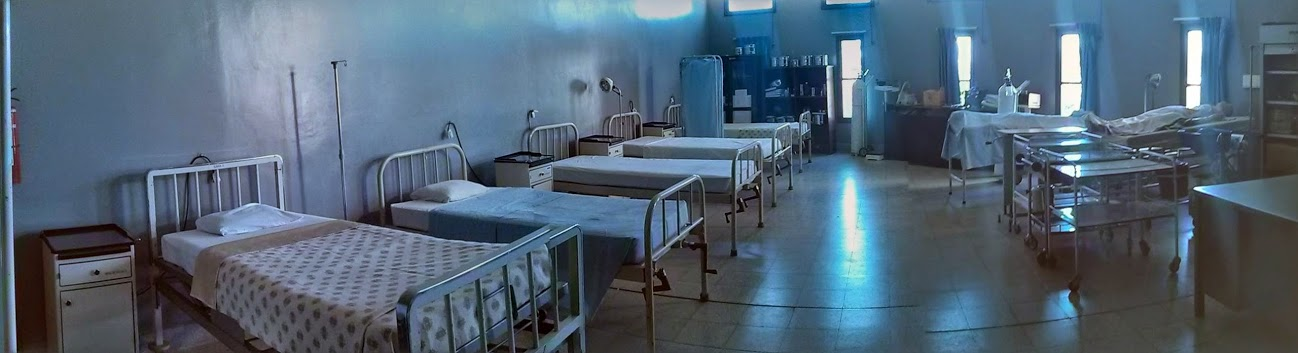
\includegraphics[scale=0.3,natwidth=100,natheight=100]{problema/iab_sala_1.jpg}
\caption{Laboratorio de enfermería del \Gls{iab}}
\label{fig:iab_lab}
\end{figure}

\fixme{Se describen}{Falta un conector} algunos de los elementos que componen al
laboratorio, estos elementos son utilizados de ejemplo para mostrar como se
lleva a cabo la práctica.

\pregunta{No se como decir que hay más elementos pero no es importante
    describirlos todos. Respuesta: Poner `entre otros materiales de uso común?`,
    al final del siguiente párrafo}

El maniquí que se observa en la figura~\ref{fig:iab_mani}, tiene ciertas
características que facilitan la práctica, por ejemplo, tiene un esquema de los
vasos sanguíneos en ambos brazos. Este maniquí se utiliza además para mostrar
las partes del cuerpo donde se puede realizar la venopunción, para mostrar la
zona específica donde se debe realizar la reanimación, y otras zonas importantes
para la práctica de enfermería.

\observacio{En algún lugar hay que mencionar las limitaciones de la simulación
    (virtual) en comparación.}

\begin{figure}[h!t] 
\centering 
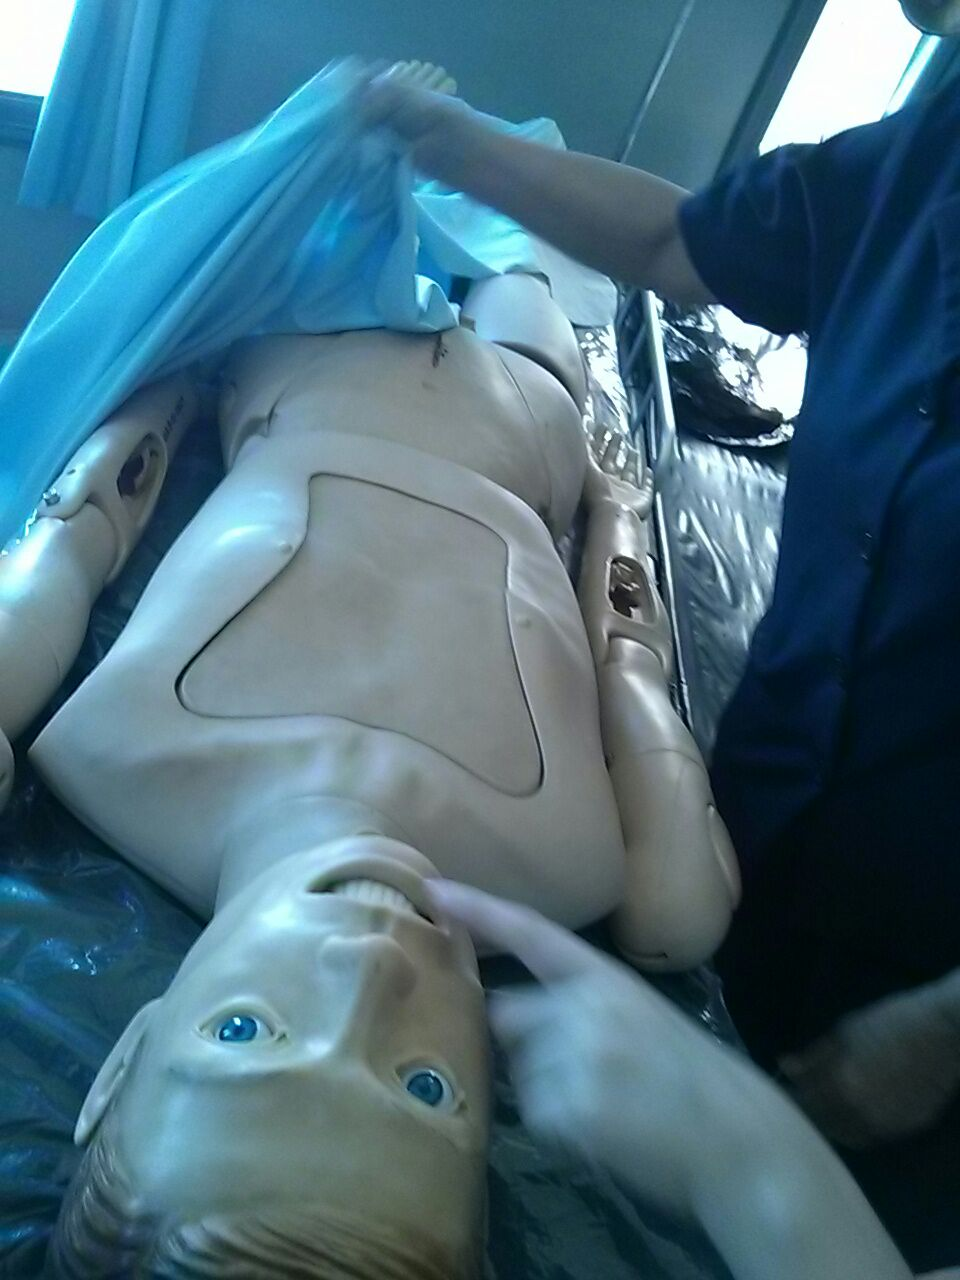
\includegraphics[scale=0.2,natwidth=400,natheight=200]{problema/iab_sala_3.jpg}
\caption{Una instructora de laboratorio muestra las partes del maniquí utilizado
    para en el laboratorio de enfermería.}
\label{fig:iab_mani}
\end{figure}

Además existen varias camas de hospitales (como se observa en la
figura~\ref{fig:iab_lab} a la izquierda), donde se practica la higienización del
paciente, como utilizar los mecanismos de ajuste de la cama, las diferentes
telas utilizadas para las sabanas, y otros aspectos relacionados al cuidado de
un paciente en cama.
